\subsection{DLR confined jet high pressure combustor}
%%%%%%%%%%%%%%%%%%%%%%%%%%%%%%%%%%%%%%%%%%%%%%%%%%%%%

The \href{https://develop.openfoam.com/exafoam/wp2-validation/-/tree/master/combustion/XiFoam/DLRCJH?ref_type=heads}{DLR confined jet high pressure combustor} stems from an experimental setup constructed by Severin at the Institute of Combustion Technology of the German Aerospace Center (abbreviated as DLR in German). The burner is based on the Recirculation-Stabilized Jet Flame (RSJF) concept, which is better known as FLOX. Initially developed for the industrial furnaces, this technology has a great potential in the application to the gas turbines. Compared to widespread swirl burners, RSJF combustors feature low NOx emissions, homogeneous temperature distribution, and operate with a wide range of fuels and loads. The main goal of the experimental work was to clarify how the recirculation contributes to the flow stabilization. Apart from the experiments, a number of numerical investigations with the same geometry was performed.

The considered combustor stems from an experimental setup constructed by Severin\footnote{\url{https://doi.org/10.18419/opus-9573}} at the Institute of Combustion Technology of the German Aerospace Center (DLR). The burner is based on the Recirculation-Stabilized Jet Flame (RSJF) concept, better known as FLOX. This technology, initially developed for industrial furnaces, has great potential in gas turbine applications. Compared to widespread swirl burners, RSJF combustors feature low NOx emissions, homogeneous temperature distribution, and operate with a wide range of fuels and loads. The main goal of the experimental work was to clarify how recirculation contributes to flow stabilization.

\begin{figure}[H]
    \centering
    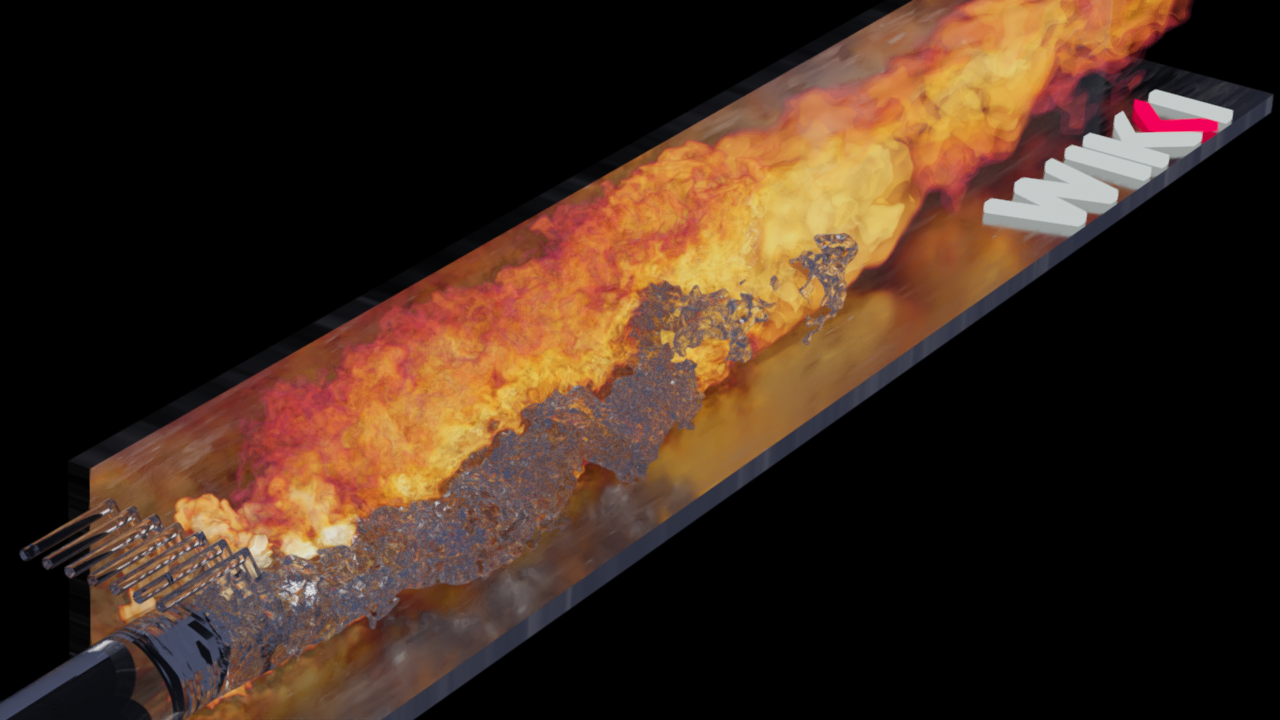
\includegraphics[width=\textwidth]{figs/DLRCJH/renderingDLRCJH.png}
    \caption{Rendering of the DLRCJH combustor flame with fuel.}
\end{figure}

\section*{Experimental Setup}
\begin{figure}[H]
    \centering
    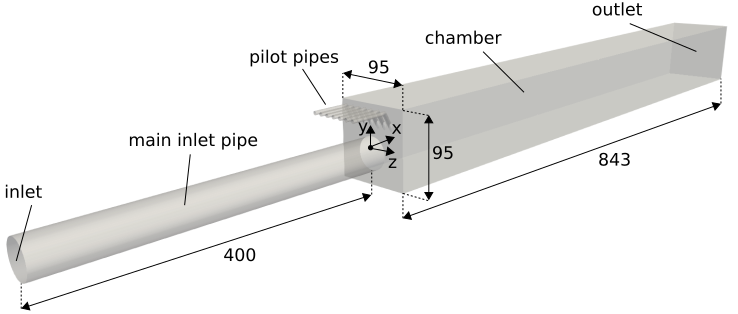
\includegraphics[width=\textwidth]{figs/DLRCJH/geometry_3D.png}
    \caption{Geometry of the combustor DLRCJH. Dimensions are in mm.}
\end{figure}

A typical RSJF combustor consists of several nozzles arranged in a ring around a central pilot swirl-burner. The test rig considered here represents a segment of such an RSJF combustor with a single nozzle\footnote{\url{https://doi.org/10.18419/opus-9573}}. It consists of a rectangular chamber with dimensions $95 \times 95 \times 843 \, \text{mm}^3$, a cylindrical inlet with a 40 mm diameter, a fuel injector placed 400 mm upstream of the chamber, and an outlet at the end of the chamber. The main inlet pipe axis is offset to the chamber centerline by 10 mm to allow for the recirculation zone to develop. The effect of the swirl-burner is simulated by seven pilot burners inclined to the main inlet axis and placed above the main inlet pipe. A premixed mixture of air and natural gas is injected through the main and pilot nozzles, where the overall mass flow of the pilots corresponds to 10\% of the main nozzle.

\section*{Measurements}
Severin\footnote{\url{https://doi.org/10.18419/opus-9573}} applied the following measurement techniques: OH*-chemiluminescence (identification of the flame position), Particle Image Velocimetry (PIV, flow speed determination), and Laser-Induced Fluorescence of the OH radical (LIF, temperature determination). The temperature and velocity fields from the middle slice (x-y plane) of the chamber were evaluated and are used here for validation.

\section*{Flow Parameters}
\begin{itemize}
    \item Reynolds number: 497,000;
    \item Average velocity at the main inlet: $\left| U_i \right| = 113 \, \text{m/s}$;
    \item Chamber pressure: 8 bar;
    \item Air-fuel ratio: 1.7;
    \item Inlet temperature of the mixture: $T_i = 725 \, K$;
    \item Adiabatic flame temperature: $1950 \, K$.
\end{itemize}

\section*{Numerical Setup}

\subsection*{Geometry}
The geometry parameters shown in the table below are taken from Severin\footnote{\url{https://doi.org/10.18419/opus-9573}}.

\begin{table}[H]
    \centering
    \begin{tabular}{ll}
        \hline
        Dimension & Description \\ \hline
        $d_i = 40 \, \text{mm}$ & Inlet nozzle diameter \\
        $y_i = -10 \, \text{mm}$ & Vertical offset of the nozzle mounting point \\
        $a = 95 \, \text{mm}$ & Lateral, top, and bottom wall width of the chamber \\
        $l = 843 \, \text{mm}$ & Chamber length \\
        $x_{inj} = -400 \, \text{mm}$ & Location of the fuel injection \\
        $d_o = 58.8 \, \text{mm}$ & Outlet nozzle diameter \\
        $d_p = 4.7 \, \text{mm}$ & Pilot nozzle diameter \\
        $\alpha = 60^\circ$ & Inclination angle of the pilot nozzles to the inlet nozzle axis \\
        $\Delta z_p = 10 \, \text{mm}$ & Distance between neighboring pilot nozzles \\
        $y_p = 25 \, \text{mm}$ & Vertical offset of the pilot nozzles mounts \\ \hline
    \end{tabular}
\end{table}

\subsection*{Initialization}
The flow is initialized either by means of *setFields* or *mapFieldsPar*. The former is used when no field data from a run of lower resolution is available. Utility *mapFieldsPar* is used for propagating the developed flow from cases with lower mesh resolution to higher ones, lowering the cost-to-solution.

\subsection*{Models}
\begin{itemize}
    \item Solver: **XiFoam** is used as the top-level solver. It handles unsteady compressible flow, incorporates combustion-relevant models, and is controlled by a PIMPLE loop allowing CFL numbers higher than 1.
    \item Turbulence: LES kinetic energy equation model (*kEqn*) with van Driest damping function for near-wall treatment.
    \item Combustion: The fuel mixture is inhomogeneous since the main and pilot nozzles are operated with different air-to-fuel ratios. The laminar flame speed $S_u$ is assumed to be unstrained, and a transport equation is solved for the flame wrinkling $\Xi$.
\end{itemize}

\subsection*{Numerics}
LES modeling relies on high accuracy discretization, utilizing higher-order schemes like *linear*, *limitedLinear*, and *limitedLinear01*. For velocity convection, *filteredLinear* is used. Temporal discretization uses a blending between Euler and Crank-Nicolson with a ratio of 30:70 (*crankNicolson 0.7*). Linear solvers are based on the conjugate gradients method. The PIMPLE loop has 2 outer and 1 inner corrections with 0 non-orthogonal corrections. Utility *renumberMesh* is used to reduce matrix bandwidth and accelerate linear solver execution.

\subsection*{Surface Mesh}
Surface mesh is created using FreeCAD 0.20\footnote{\url{https://wiki.freecad.org/Release_notes_0.20}}.

\subsection*{Mesh}
Meshing is accomplished with *snappyHexMesh (sHM)*. Four surface meshes are provided:
- An .obj file with the complete geometry with regions corresponding to boundaries.
- An .stl file with the complete geometry without regions.
- Two additional .stl files with surface meshes of the inlet pipe and pilots.

Four meshes with resolutions of 3M, 24M, 189M, and 489M cells have been produced successively.

\section*{Boundary Conditions}
\begin{table}[H]
    \centering
    \begin{tabular}{lllll}
        \hline
        Quantity & Main Inlet & Pilot Inlet & Walls & Outlet \\ \hline
        $\alpha_t$ & zG & zG & wF & c \\
        $b$ & fV 1 & fV 1 & zG & iO 0 \\
        $f_t$ & fV 0.03344 & fV 0.06084 & zG & iO 0.03344 \\
        $k$ & fV $1e-5$ & fV $1e-5$ & wF & iO $1e-5$ \\
        $\nu_t$ & c & c & zG & c \\
        $p$ & zG & zG & zG & wT $8e5$ 5 \\
        $S_u$ & c & c & zG & c \\
        $T$ & fV 725 & fV 633 & CF: fV 600; CL: fV 800; other: zG & iO 1000 \\
        $T_u$ & fV 725 & fV 633 & CF: fV 600; CL: fV 800; other: zG & iO 1000 \\
        $U$ & fRIV 0.5563 & fRIV 0.0558 & fV $(0, 0, 0)$ & iO $(0, 0, 0)$ \\
        $\Xi$ & fV 1 & fV 1 & zG & iO 20 \\ \hline
    \end{tabular}
\end{table}

Abbreviations:
\begin{itemize}
    \item c: calculated BC;
    \item CF: Chamber Front (baseplate);
    \item CL: Chamber Lateral walls;
    \item fRIV *massFlowRate*: flowRateInletVelocity BC;
    \item fV *value*: fixedValue BC;
    \item iO *inletValue*: inletOutlet BC;
    \item wF: wallFunction BC;
    \item wT *fieldInf* *lInf*: waveTransmissive BC;
    \item zG: zeroGradient BC.
\end{itemize}

\section*{Validation}
Validation was performed with results from Severin\footnote{\url{https://doi.org/10.18419/opus-9573}} using the case with 24 million cells. Temperature and velocity profiles were averaged over 0.05 seconds of physical time.

\begin{figure}[h]
    \centering
    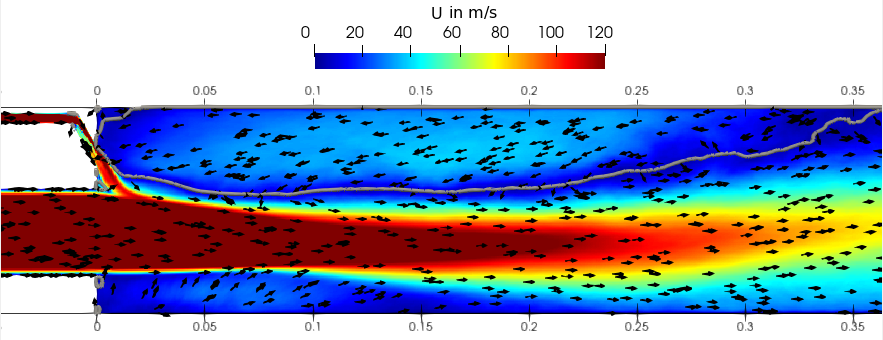
\includegraphics[width=0.8\textwidth]{figs/DLRCJH/7608d6e2c381894c3303bca616371060.png}
    \caption{Velocity comparison: Computation vs. Experiment.}
\end{figure}

\section*{Grand Challenge}
\begin{itemize}
    \item Known to run with OpenFOAM-v2106, -v2112, -v2306 compiled with double precision.
    \item Three cases are provided: 3M, 24M, and 489M.
    \item Two setups for each mesh size are provided: *fixedTol* and *fixedIter*.
\end{itemize}

\section*{Known Issues}
\begin{itemize}
    \item During meshing, a bug related to FMA instructions has been encountered.
    \item Utility *mapFieldsPar* failed to map from 189M to 489M while using collated fileHandler.
    \item Provided coded function object *FOwallClockTimeStatistics* may cause issues during startup.
\end{itemize}

\section*{Benchmark Results}
Two supercomputers were used for benchmarking: HAWK and LUMI.

\subsection*{Strong Scaling}
Normalized time to solution is calculated as $T_i^* = t_i N_c / N_e$, where $t_i$ is the time per iteration, $N_c$ is the number of cores, and $N_e$ is the number of cells.

\subsubsection*{3M Case}
\begin{figure}[h]
    \centering
%    \includegraphics[width=0.8\textwidth]{figures/speedup_3M.png}
    \caption{Speedup for the 3M case.}
\end{figure}

\subsubsection*{24M Case}
\begin{figure}[h]
    \centering
%    \includegraphics[width=0.8\textwidth]{figures/speedup_24M.png}
    \caption{Speedup for the 24M case.}
\end{figure}

\subsubsection*{489M Case}
\begin{figure}[h]
    \centering
%    \includegraphics[width=0.8\textwidth]{figures/speedup_489M_largeRunsOnly.png}
    \caption{Speedup for the 489M case.}
\end{figure}

\subsection*{Weak Scaling}
Weak scaling benchmarks were performed for loads of 60K, 30K, 15K, and 7.5K cells per core.

\section*{Coherent File Format}
The coherent format addresses major IO bottlenecks, resulting in significant improvements:
- Case decomposition: up to 60 times lower time-to-solution.
- Overall pre- and post-processing: 31 times lower cost-to-solution.
- Solver execution: 30 times lower time-to-solution.